\chapter{Reconstructing proton-proton collisions with the CMS detector}
\section{The LHC and its proton injection system}
\section{The CMS detector}
The Compact Muon Solenoid (CMS) detector is a multi-purpose apparatus which operates at the LHC. 
It is installed about 100 metres underground close to the French village of Cessy, between
Lake Geneva and the Jura mountains.

The detector requirements for CMS to meet the goals of the LHC physics programme are as follows:
\begin{itemize}
\item Good muon identification and momentum resolution over a wide range of momenta and
angles, good dimuon mass resolution (1\% at 100 GeV), and the ability to determine unambiguously
the charge of muons with p < 1 TeV
\item Good charged-particle momentum resolution and reconstruction efficiency in the inner
tracker. Efficient triggering and offline tagging of $\tau$'s and b-jets, requiring pixel detectors
close to the interaction region
\item Good electromagnetic energy resolution, good diphoton and dielectron mass resolution (1\% at 100 GeV),
wide geometric coverage, ${\pi}^{0}$ rejection, and efficient photon and lepton
isolation at high luminosities
\item Good missing-transverse-energy and dijet-mass resolution, requiring hadron calorimeters
with a large hermetic geometric coverage and with fine lateral segmentation
\end{itemize}

The central feature of the CMS apparatus is a superconducting solenoid of 6 m internal diameter, providing a magnetic field of 3.8 T.
Within the solenoid volume are a silicon pixel and strip tracker, a lead tungstate crystal electromagnetic calorimeter (ECAL), and a brass and scintillator hadron calorimeter (HCAL), each composed of a barrel and two endcap sections. 
Forward calorimeters extend the pseudorapidity coverage provided by the barrel and endcap detectors. 
Muons are detected in gas-ionization chambers embedded in the steel flux-return yoke outside the solenoid.

Events of interest are selected using a two-tiered trigger system~\cite{Khachatryan:2016bia}.
The first level, composed of custom hardware processors, uses information from the calorimeters and muon detectors to select events at a rate of around 100 kHz within a time interval of less than 4 $\mu$s.
The second level, known as the high-level trigger, consists of a farm of processors running a version of the full event reconstruction software optimized for fast processing, and reduces the event rate to around 1 kHz before data storage.
\subsection{Trackers}

The inner tracking system of CMS is designed to provide a precise and efficient measurement
of the trajectories of charged particles emerging from the LHC collisions, as well as a precise
reconstruction of secondary vertices. It surrounds the interaction point and has a length of 5.8 m
and a diameter of 2.5 m. The CMS solenoid provides a homogeneous magnetic field of 4 T over
the full volume of the tracker.
At the LHC design luminosity of 1034 cm\textsuperscript{-2} s\textsuperscript{-1},
there are on average about 1000 particles from more than 20 overlapping proton-proton interactions traversing
the tracker for each bunch crossing, i.e. every 25 ns. Therefore, a detector technology featuring high
granularity and fast response is required, such that the trajectories can be identified reliably and
attributed to the correct bunch crossing. However, these features imply a high power density of
the on-detector electronics which in turn requires efficient cooling. This is in direct conflict with
the aim of keeping to the minimum the amount of material in order to limit multiple scattering,
bremsstrahlung, photon conversion and nuclear interactions. A compromise had to be found in this
respect. The intense particle flux will also cause severe radiation damage to the tracking system.
The main challenge in the design of the tracking system was to develop detector components able
to operate in this harsh environment for an expected lifetime of 10 years. These requirements on
granularity, speed and radiation hardness lead to a tracker design entirely based on silicon detector
technology. The CMS tracker is composed of a pixel detector with three barrel layers at radii
between 4.4 cm and 10.2 cm and a silicon strip tracker with 10 barrel detection layers extending
outwards to a radius of 1.1 m. Each system is completed by endcaps which consist of 2 disks in
the pixel detector and 3 plus 9 disks in the strip tracker on each side of the barrel, extending the
acceptance of the tracker up to a pseudorapidity of $|\eta| < 2.5$. With about 200 m\textsuperscript{2} of active silicon
area the CMS tracker is the largest silicon tracker ever built.

\subsection{Electromagnetic calorimeter}
The electromagnetic calorimeter of CMS (ECAL) is a hermetic homogeneous calorimeter made of
61 200 lead tungstate ($\textrm{PbWO}_{\textrm{4}}$) crystals mounted in the central barrel part, closed by 7 324 crys-
tals in each of the two endcaps. A preshower detector is placed in front of the endcap crystals.
Avalanche photodiodes (APDs) are used as photodetectors in the barrel and vacuum phototriodes
(VPTs) in the endcaps. The use of high density crystals has allowed the design of a calorimeter
which is fast, has fine granularity and is radiation resistant, all important characteristics in the LHC
environment. One of the driving criteria in the design was the capability to detect the decay to two
photons of the postulated Higgs boson. This capability is enhanced by the good energy resolution
provided by a homogeneous crystal calorimeter.

\subsection{Hadron calorimeters}
The hadron calorimeters (HCALs) are particularly important for the measurement of hadron jets and neutrinos or exotic particles resulting in apparent missing transverse energy \cite{CMSTDR}.
Figure~\ref{fig:hcalslice} shows the longitudinal view of the CMS detector. The dashed lines are at fixed $\eta$ values. 
The hadron calorimeter barrel and endcaps sit behind the tracker and the electromagnetic
calorimeter as seen from the interaction point. The hadron calorimeter barrel is radially restricted
between the outer extent of the electromagnetic calorimeter (R = 1.77 m) and the inner extent of
the magnet coil (R = 2.95 m). This constrains the total amount of material which can be put in
to absorb the hadronic shower. Therefore, an outer hadron calorimeter or tail catcher is placed
outside the solenoid complementing the barrel calorimeter. Beyond $|\eta| = 3$, the forward hadron
calorimeters placed at 11.2 m from the interaction point extend the pseudorapidity coverage down
to $|\eta| = 5.2$ using a Cherenkov-based, radiation-hard technology.
The HCAL subsystems are described briefly below, with more detailed information on the geometry and 
readout being available in~\cite{CMSTDR}.
\begin{figure}
\centering
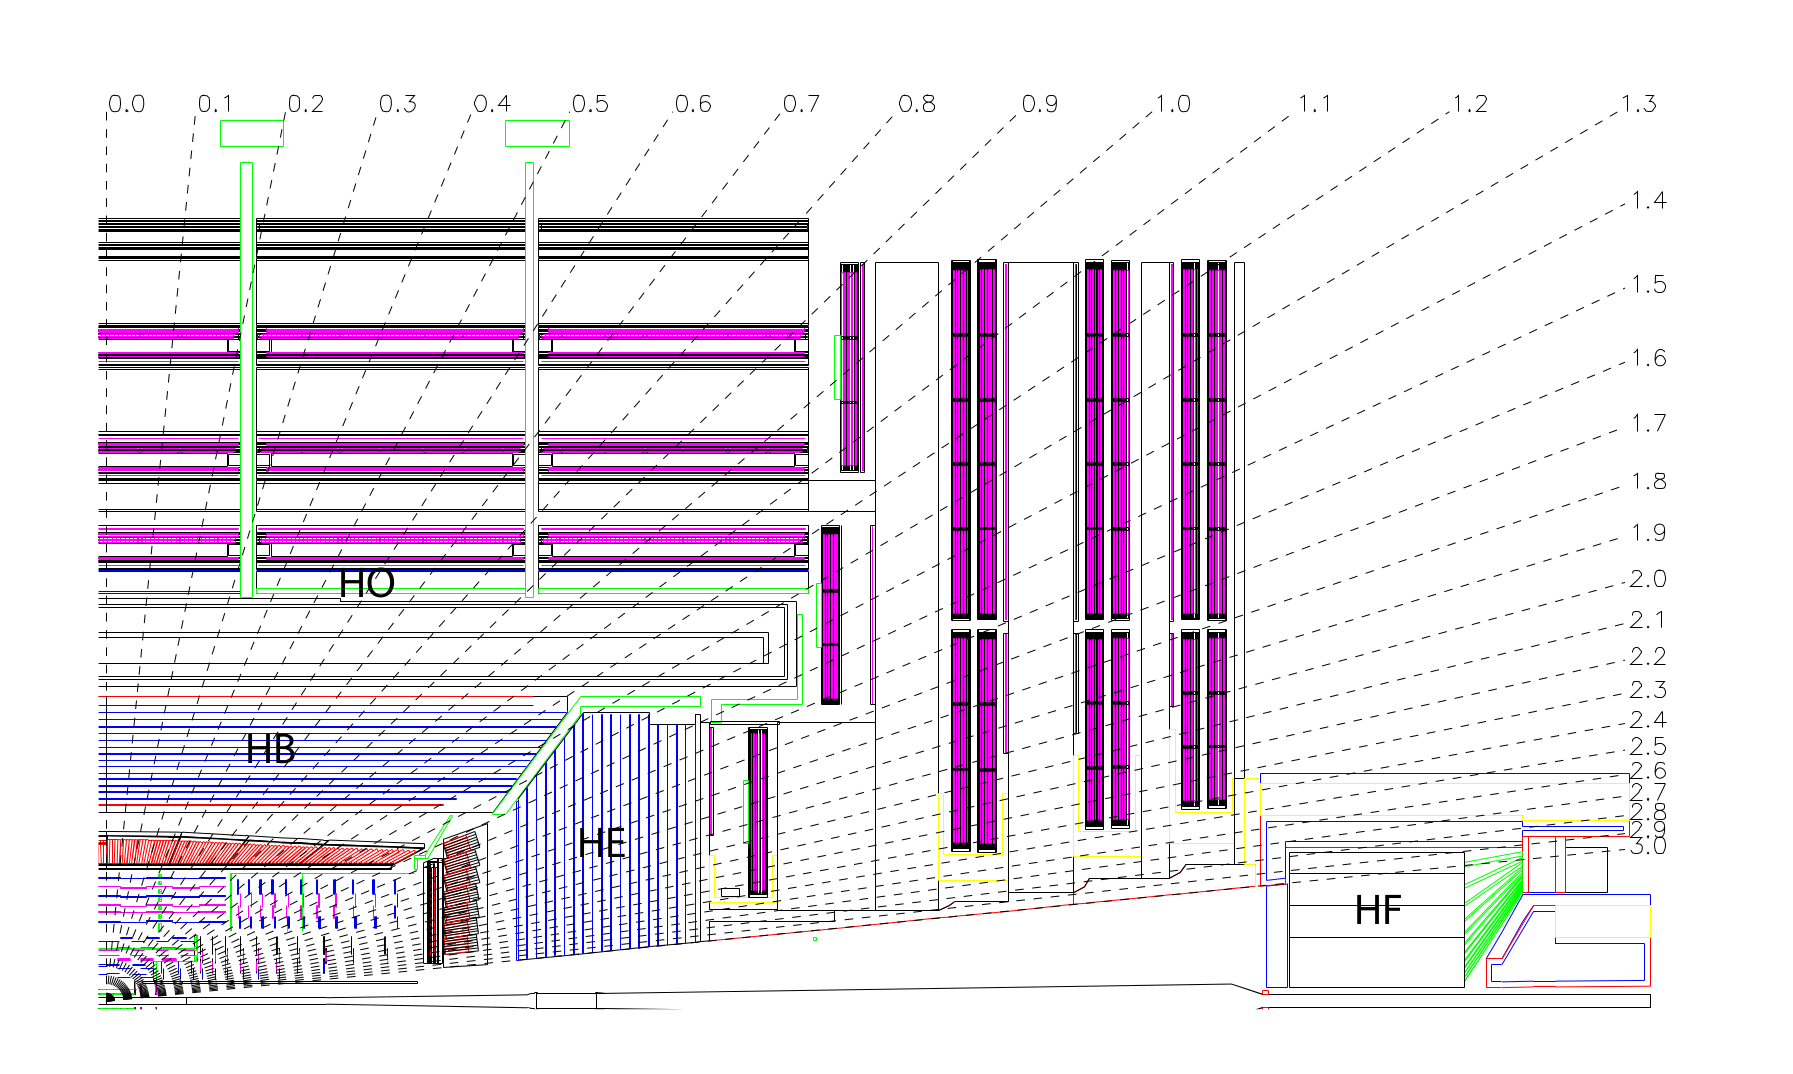
\includegraphics[width=0.98\textwidth,natwidth=1793,natheight=1074]{figures/hcalslice.png}
\caption{Longitudinal slice of the CMS detector showing the locations of the hadron barrel
(HB), endcap (HE), outer (HO) and forward (HF) calorimeters.}
\label{fig:hcalslice}
\end{figure}

\subsubsection{HCAL barrel}
The HCAL barrel (HB) is a sampling calorimeter and covers the pseudorapidity range $|\eta| < 1.3$.
It consists of 36 identical azimuthal wedges which form two half-barrels. 
The wedges are constructed out of flat brass absorber plates which are parallel
to the beam axis.  Each wedge is segmented into four azimuthal angle ($\phi$) sectors. 
The innermost and outermost plates are made of stainless steel for structural strength.

The absorber consists of a front steel plate 40 mm thick,
followed by eight 50.5 mm thick brass plates, six 56.5 mm thick brass plates,
and a 75 mm thick steel back plate.
The last layer is thicker to correct for late developing showers which could leak out the back.
The total absorber thickness at 90\textdegree~is 5.82 interaction lengths ($\lambda_I$).
The HB effective thickness increases with polar angle ($\theta$) as $1/\textrm{sin}\:\theta$,
resulting in 10.6 $\lambda_I$ at $|\eta| = 1.3$. 

The HB baseline active material is 3.7 mm thick Kuraray SCSN81 plastic scintillator, 
chosen for its long-term stability and moderate radiation hardness. 
The first layer of scintillator is located in front of the steel support plate, 
and is made of 9 mm thick Bicron BC408. 
Its purpose is to sample hadronic showers developing in the inert material between
the ECAL barrel and the HCAL barrel.
The plastic scintillator is divided into 16 $\eta$ sectors, resulting in a segmentation of $(\Delta\eta, \Delta\phi) = (0.087, 0.087)$. 

\subsubsection{HCAL endcaps}

The hadron calorimeter endcaps (HE) cover the rapidity range $1.3 < |\eta| < 3$. 
It is designed for high radiation tolerance, in order to survive 10 MRad after 10 years of operation.
The total length of the endcap calorimeter, after the ECAL and HCAL endcaps, is about 10 interaction lengths. 

The absorber is made of C26000 cartridge brass, due to its mechanical properties, its high number of interaction lengths, and its relatively low cost.
Furthermore, it may sit in the 4 T axial magnetic field.
The absorber is assembled in a staggered geometry which minimizes the cracks between HB and HE and contains no projective dead material. 

The scintillators are of trapezoidal shape and there are 18 layers of them in total. 
The first layer are made of 9 mm thick Bicron BC408. All the rest are made of 3.7 mm thick SCSN81.
The scintillation light is read out via wavelength shifting fibers. 
The granularity of the calorimeters is $(\Delta\eta, \Delta\phi) = (0.087, 0.087)$ for $|\eta| < 1.6$ and $(\Delta\eta, \Delta\phi) = (0.170, 0.170)$ for $|\eta| \geq 1.6$.

\subsubsection{HCAL outer}
The combined stopping power of the ECAL and HCAL barrels does not provide adequate stopping
power in the central region $|\eta| < 1.3$. This is problematic for the missing energy resolution.
To further measure and contain these showers, the hadron calorimeter is extended outside the solenoid with a tail catcher called the HO. Only 40 mm of space in the radial direction is available, 
24 mm of which is used for aluminum honeycomb support structures.

The scintillator plates of the HO are made of 10 mm thick Bicron BC408. There are 5 rings in $\eta$, each of those rings having 12 identical $\phi$ sectors, and each of those sectors having 6 azimuthal slices.
The sizes and positions of the tiles in HO are supposed to roughly map the layers of HB
to make towers of granularity $(\Delta\eta, \Delta\phi) = (0.087, 0.087)$.

The magnetic solenoid coil is used as an additional absorber equal to $1.4/\textrm{sin}\:\theta$ interaction lengths.
Outside the vacuum tank, the magnetic field is returned through an iron yoke roughly 20 mm thick, with 5 rings corresponding to the scintillator plates.
The central ring has scintillators both inside and outside of the iron yoke ring.
The others have scintillators only outside their yoke rings.
All told, the total depth of the calorimeter system is extended to a minimum of
$11.8\:\lambda_I$ except at the barrel-endcap boundary region.

\subsubsection{HCAL forward}
The forward calorimeter, or HF, exists in an extremely hostile environment. 
At $|\eta|=5$ we expect to have delivered 10 MGy after 10 years of operation.
The active material is fused-silica core, polymer hard-cladded quartz fibers, which have sufficient radiation hardness.
These fibers measure 600 $\pm$ \SI{10}{\micro\meter} in diameter for the fused-silica core,
$ {630}^{+5}_{-10}$ \SI{}{\micro\meter} with the polymer hard-cladding, 
and 800 $\pm$ \SI{30}{\micro\meter} with the protective acrylate buffer.

The geometry consists of a steel absorber structure composed of 5 mm thick grooved
plates. Fibers are inserted in these grooves.
The detector is functionally subdivided into two longitudinal segments. 
Half of the fibers run over the full depth of the absorber (165 cm $\approx 10\:\lambda_I$)
while the other half starts at a depth of 22 cm from the front of the detector.
These two sets of fibers are read out separately. 
This arrangement makes it possible to distinguish showers generated by electrons and photons,
which deposit a large fraction of their energy in the first 22 cm,
from those generated by hadrons, which produce nearly equal signals in both calorimeter segments on average. 
The absorber has grooves which make a square grid separated by 5.0 $\pm$ 0.1 mm center-to-center, with long and short fibers alternating in the grooves. 

This calorimeter is mostly sensitive to the electromagnetic component of hadronic showers.
Only light that hits the core-cladding interface at an angle larger than the critical angle (71\textdegree) contributes to the calorimeter signal in the form of Cherenkov light. 
After the quoted 10 MGy dose has accumulated over the HF lifetime, the optical transmission of the fibers is reduced just by a factor of 2.

\subsection{Muon systems}

\begin{figure}
\centering
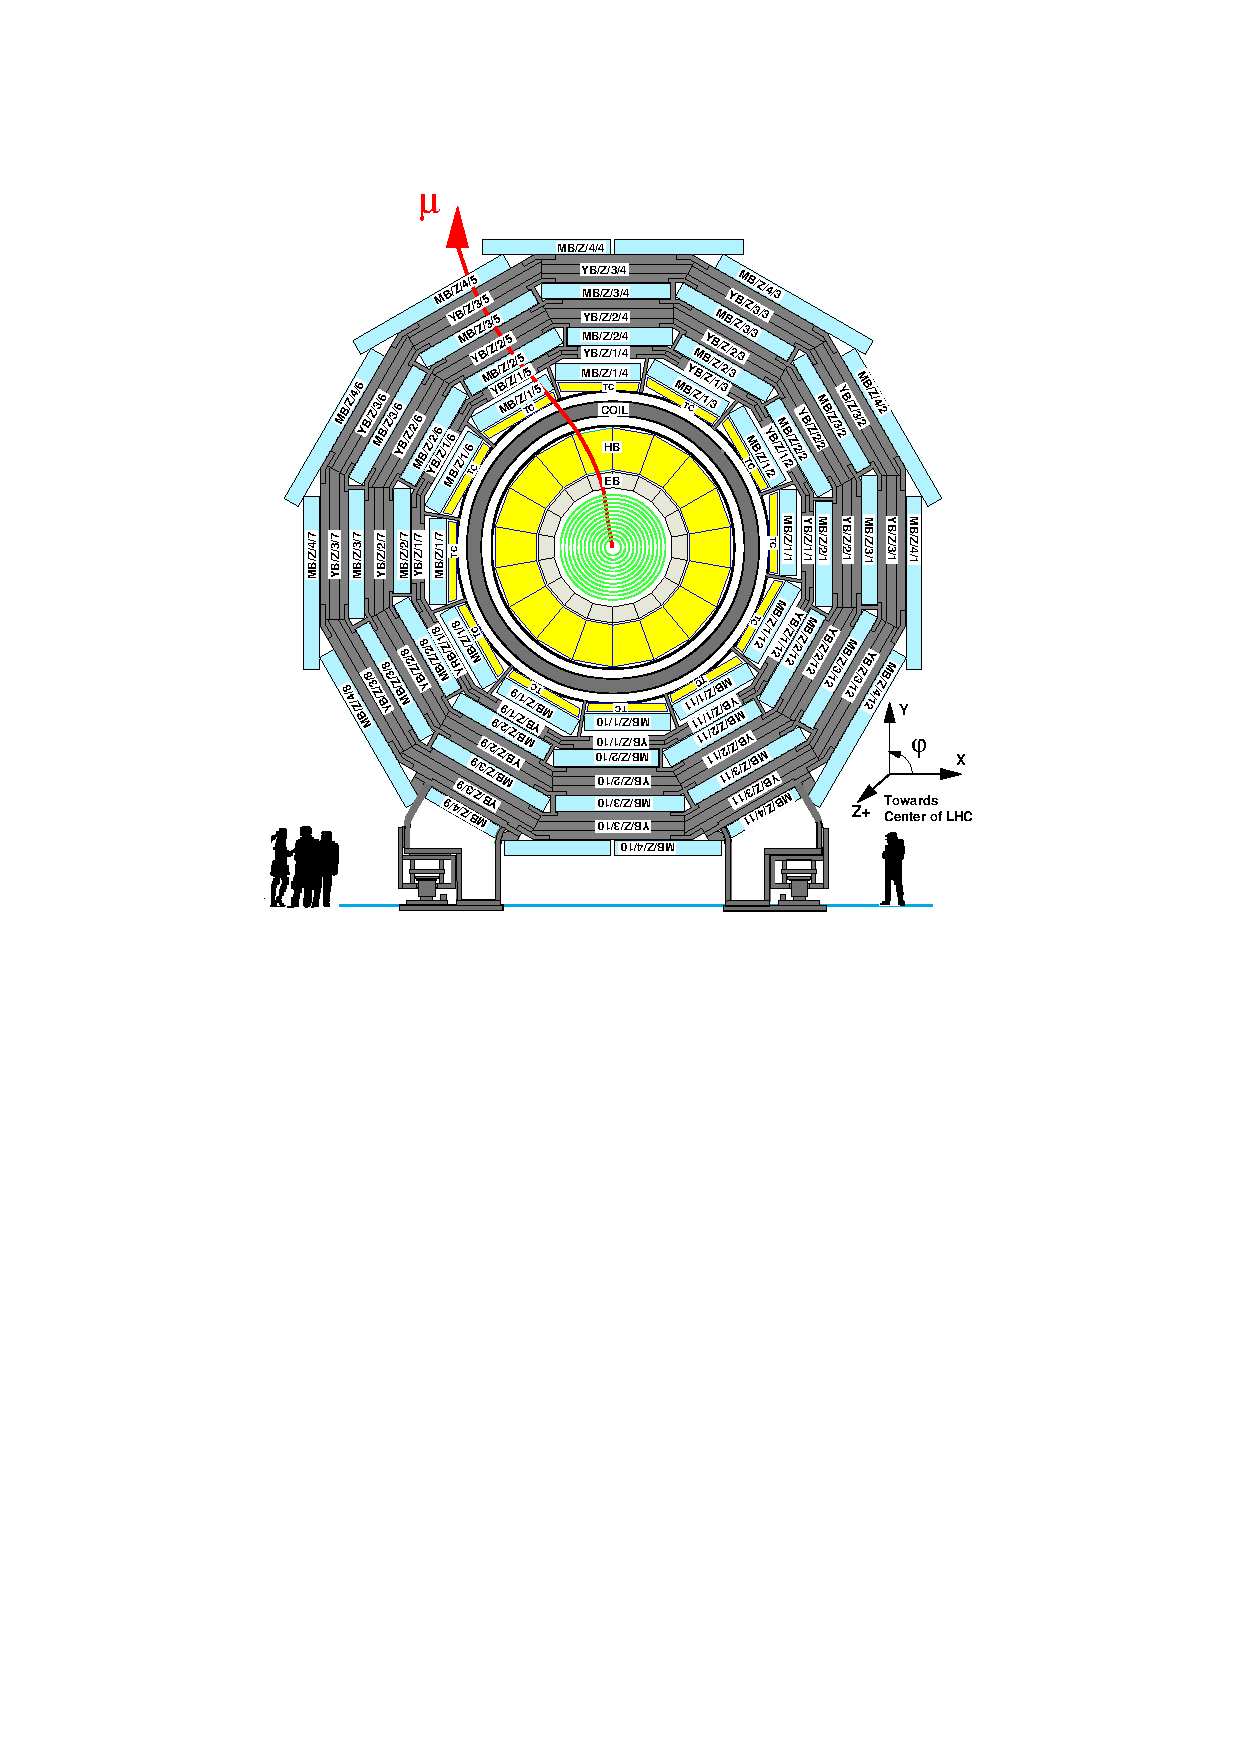
\includegraphics[width=0.5\textwidth]{figures/cms_drifttubes_slice.pdf}
\caption{
Layout of the CMS barrel muon DT chambers in one of the 5 wheels. The chambers in
each wheel are identical with the exception of wheels –1 and +1 where the presence of cryogenic
chimneys for the magnet shortens the chambers in 2 sectors.
}
\label{fig:dtslice}
\end{figure}

\begin{figure}
\centering
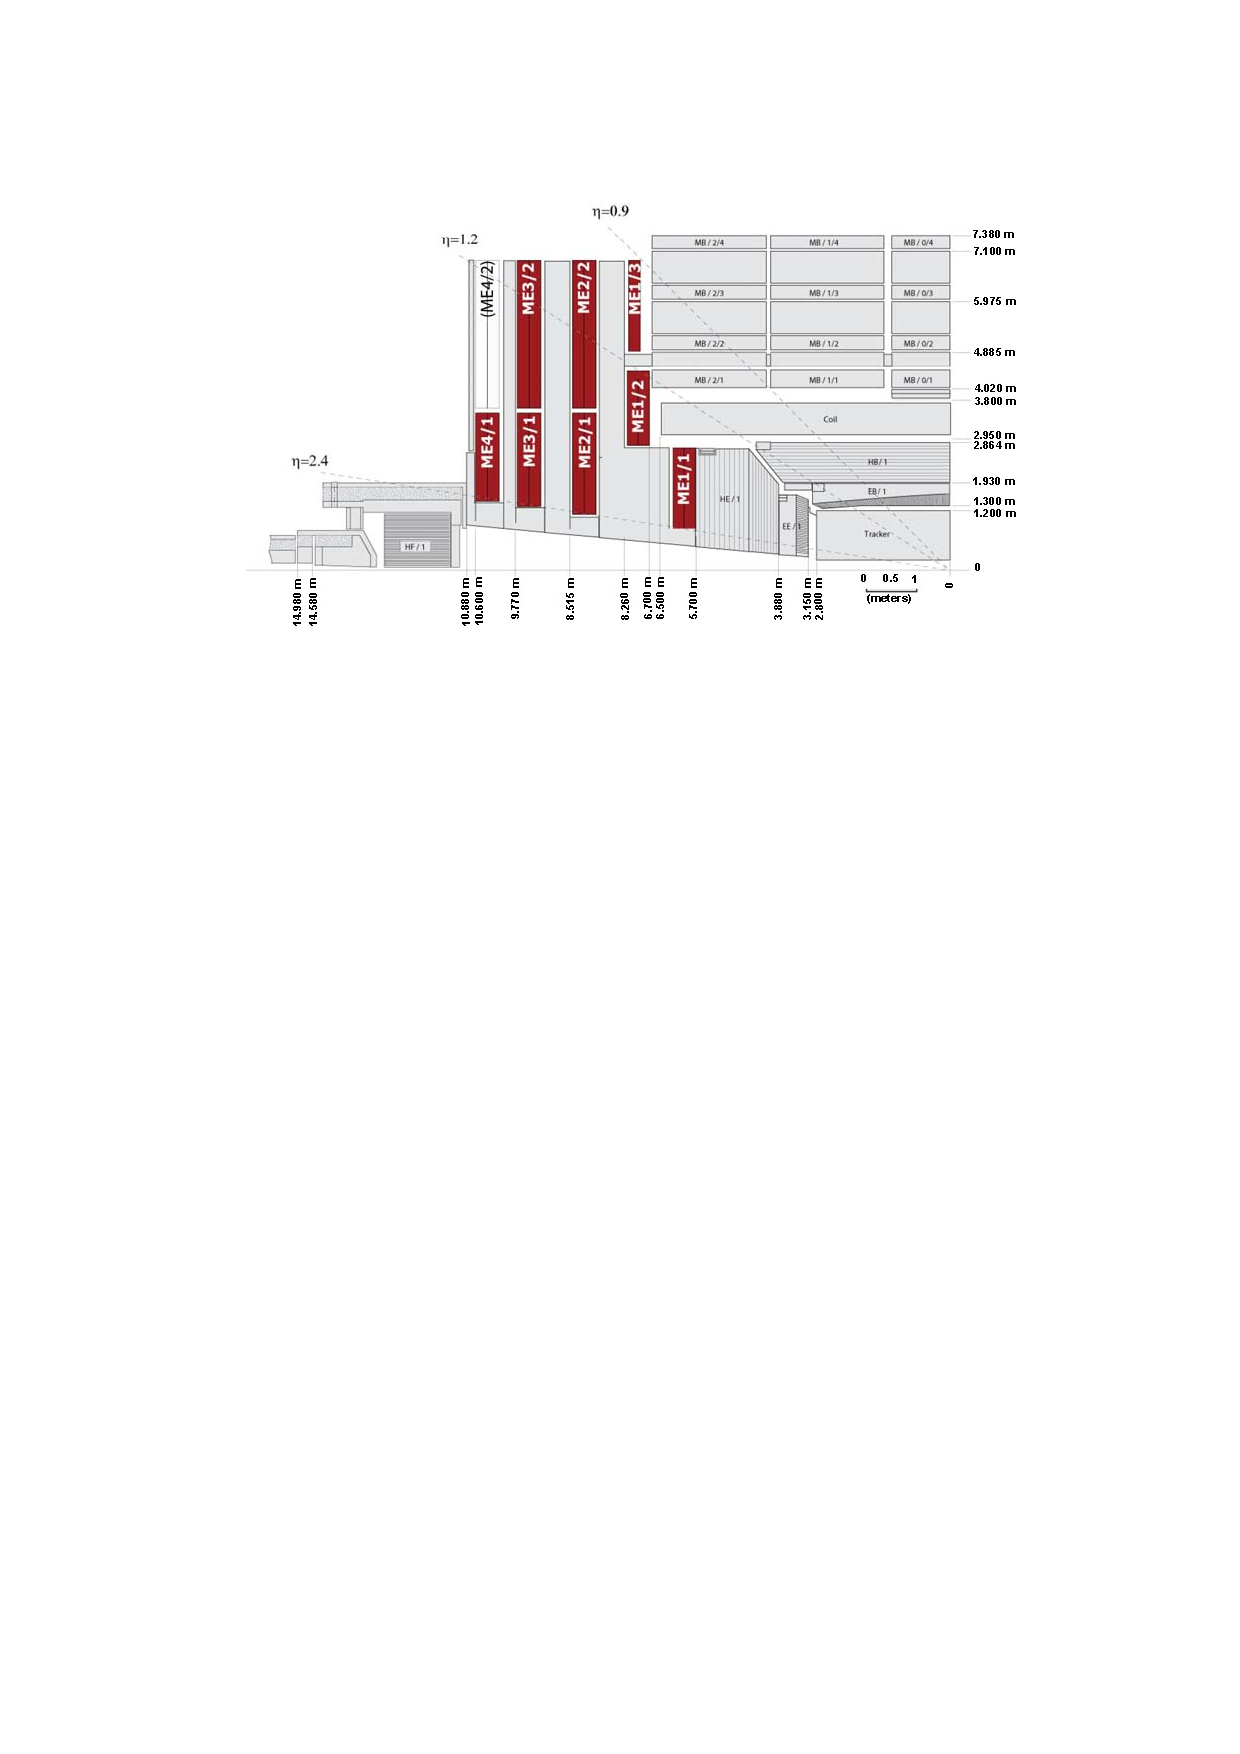
\includegraphics[width=0.5\textwidth]{figures/cms_quarter_csc_red.pdf}
\caption{
Quarter-view of the CMS detector. Cathode strip chambers of the Endcap Muon
system are highlighted.
}
\label{fig:cms_quarter_csc_red}
\end{figure}

\begin{figure}
\centering
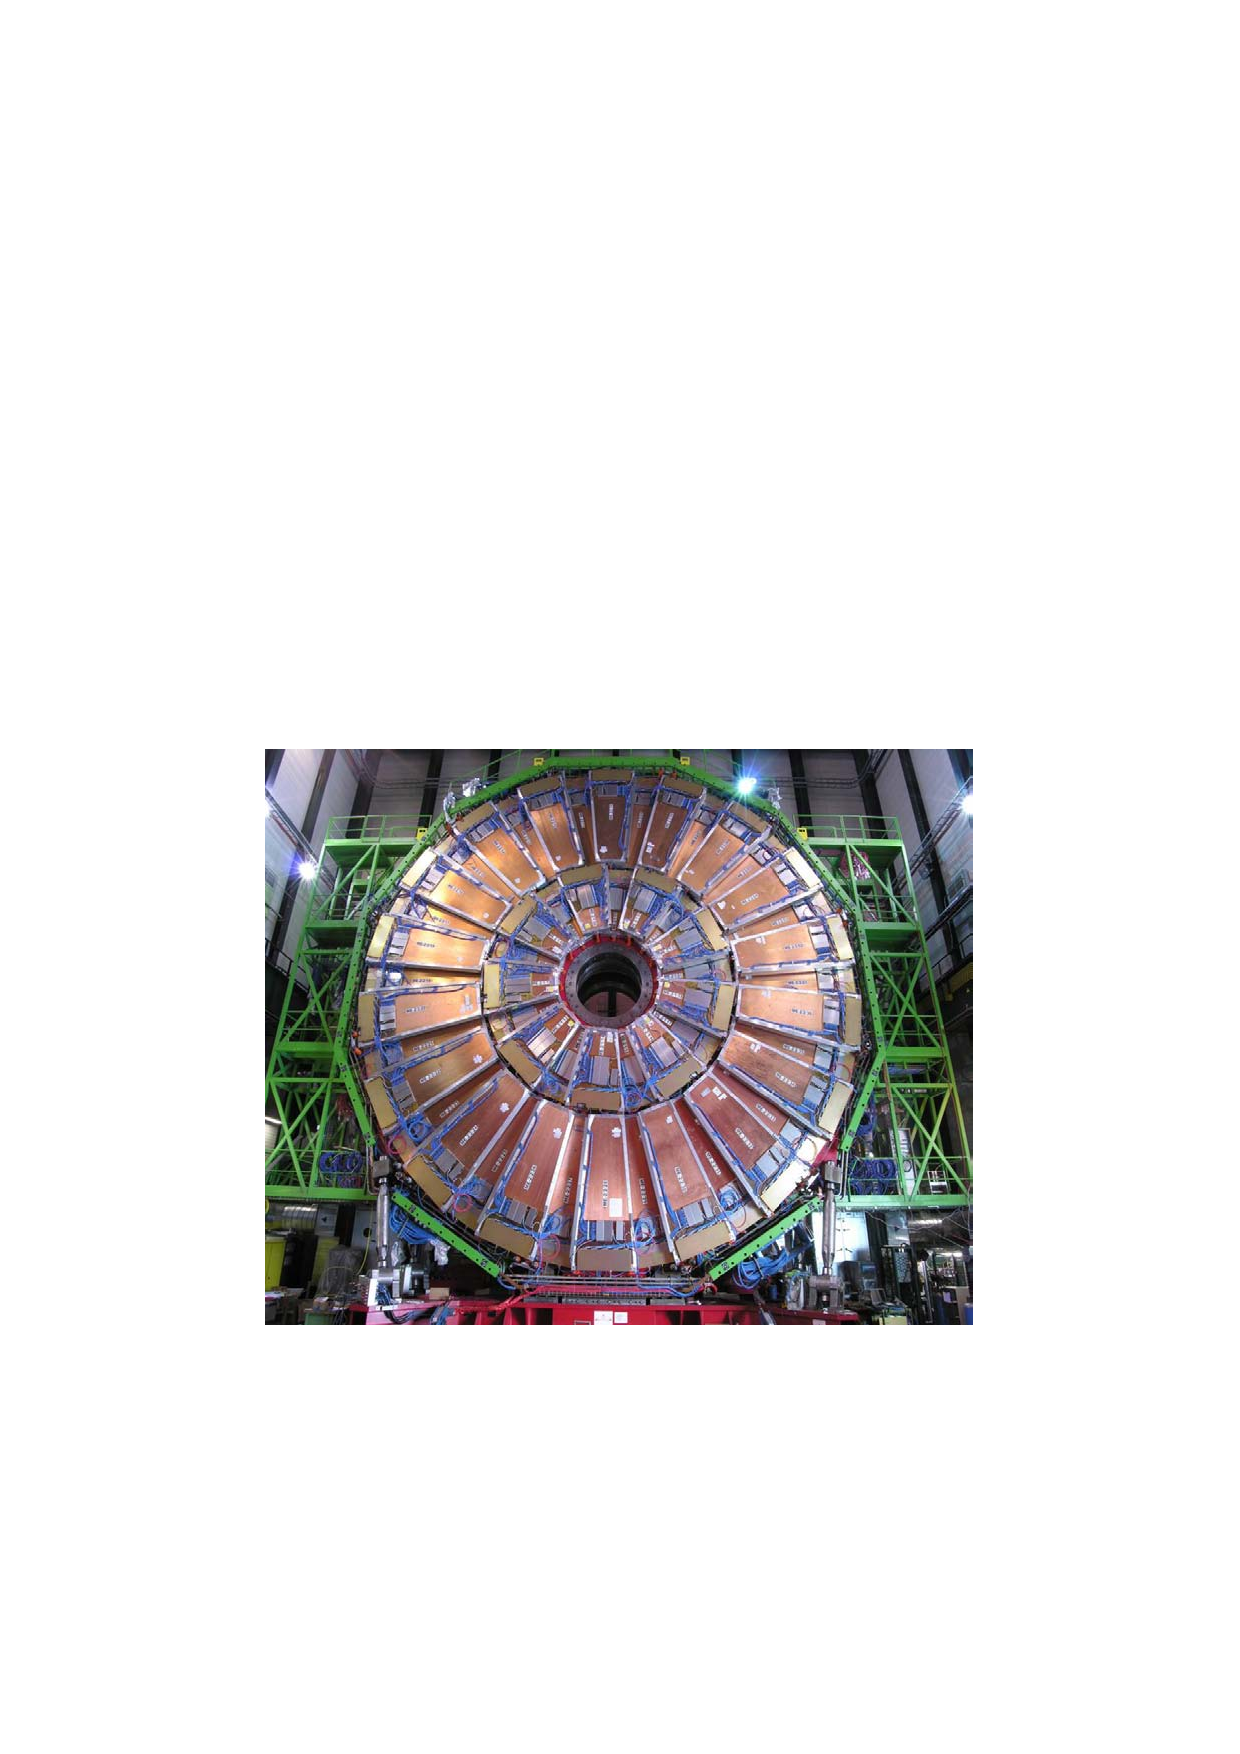
\includegraphics[width=0.5\textwidth]{figures/cms_cscs_me2.pdf}
\caption{
The ME2 station of CSCs. The outer ring consists of 36 ME2/2 chambers, each
spanning 10\degree in \phi, and the inner ring of eighteen 20\degree ME2/1 chambers.
The chambers overlap to provide contiguous coverage in \phi.
}
\label{fig:cms_cscs_me2}
\end{figure}



\section{Object reconstruction}
\subsection{Electrons}
Electrons in the CMS detector are reconstructed through association of a track from the silicon detector with a cluster of energy in the ECAL.
Electron tracks are formed from initial seeds likely to correspond to initial electron trajectories, which are then used to build tracks by collecting hits in the silicon tracker using the combinatorial Kalman filter procedure.
Next, a track fitting procedure is undertaken using a Gaussian Sum Filter (GSF), in which the energy loss in each tracker layer is approximated by a mixture of Gaussian distributions.
Meanwhile, the electron energy has been collected in several crystals of the ECAL. 
These depositions undergo two steps of clustering.
The first step finds clusters from crystal arrays of $5 \times 1$ in $\eta \times \phi$ for the ECAL barrel, and $5 \times 5$ crystals for the ECAL endcaps.
The second step forms a supercluster (SC) comprising the energy of constituent clusters.
The supercluster position and energy, along with the GSF track, reconstruct the electron in the detector.\cite{ElectronReco2015}
The reconstruction procedure is also informed by the Particle-Flow algorithm, described later in Section ???.

The final electron momentum is found using a multivariate regression tuned on simulation to give better energy resolution.
A residual energy scale correction is applied to the reconstructed electrons based on time, electron $\eta$, and shower shape variables
such that the Z mass peak resolution is enhanced.  In addition, a smearing is applied to simulation such that the energy resolution in data and simulation match.

The isolation of the lepton candidates is computed from the flux of particle flow candidates
found within a cone of $\Delta R = 0.4$ built around the lepton direction~\cite{CMS-PAS-PFT-10-002}.
The flux of particles is computed independently for the charged hadrons, neutral hadrons and photon candidates.
The contribution from neutral hadron candidates is corrected for the influence of PU by using the \textit{effective area} approach.  The average energy density per area due to PU ($\rho$) is multiplied with an effective area ($A_{\rm eff}$) and subtracted from the isolation sum. $A_{\rm eff}$ is chosen in such a way that the isolation is independent of the number of pileup interactions.
The relative electron isolation sum is defined as: 

\begin{equation}
I^{e}_{\rm rel}=\frac{1}{p_{\rm T}}  \left[ I_{\rm ch}+\max(I_{\rm nh}+I_{\rm g}-A_{\rm eff}\cdot\rho,0) \right]
\label{eq:eleisol}
\end{equation}

\subsection{Muons}
Muon tracks are reconstructed in the CMS detector in both the silicon tracker and the muon spectrometer,
resulting respectively in tracker tracks and standalone-muon tracks.
Subsequently, these tracks inform two reconstruction approaches:
\begin{enumerate}
  \item {\em Global Muon reconstruction (outside-in):} starting from a standalone
    muon in the muon system, a matching tracker track is found and a
    {\em global-muon track} is fitted combining hits from the tracker track
    and standalone-muon track. At large transverse momenta ($\pt \gsim 200$~GeV/$c$),
    the global-muon fit can improve the momentum resolution compared
    to the tracker-only fit. 
  \item {\em Tracker Muon reconstruction (inside-out):} in this approach, all
    tracker tracks with $\pt >$ 0.5~GeV/$c$ and $p >$ 2.5~GeV/$c$ are
    considered as possible muon candidates and are extrapolated to the muon system, taking into
    account the expected energy loss and the uncertainty due to multiple
    scattering. If at least one muon segment (i.e. a short track stub made of DT or CSC hits)
    matches the extrapolated track,
    the corresponding tracker track qualifies as a {\em tracker-muon track}.
    The extrapolated track and the segment are considered to be matched if the distance
    between them in local $x$ is less than 3~cm or if the value of the pull
    for local $x$ is less than 4.
    At low momentum (roughly $p < 5$~GeV/$c$) this approach is more
    efficient than the global muon 
    reconstruction, since it requires only a single muon segment in
    the muon system, whereas global muon reconstruction is designed to have
    high efficiency for muons penetrating through more than one muon station.
\end{enumerate}

The majority of muons from collisions (with sufficient momentum) are reconstructed either 
as a Global Muon or a Tracker Muon, or very often as both.
A third, rare case is excluded from this note, where both approaches fail and only a {\em standalone-muon track} is found~\cite{CMS-PAS-MUO-10-004}.

For the muon isolation, in the same manner as for electrons, a cone of $\Delta R = 0.4$ is built to compute the flux of particle flow candidates,
the ``delta-beta'' correction is applied to correct for pileup contamination. This correction is achieved by
subtracting half the sum of the \pt of the charged particles in the cone of interest but with particles not originating from the primary vertex.
The muon isolation is therefore defined as:

\begin{equation}
I^{\mu}_{\rm rel}=\frac{1}{p_{\rm T}}  \left[ I_{\rm ch}+\max(I_{\rm nh}+I_{\rm g}-0.5\cdot I_{\rm chPU} ,0) \right]
\label{eq:muisol}
\end{equation}

The factor $0.5$ corresponds to a approximate average of neutral to charged particles and has been measured in jets in~\cite{CMS-PAS-PFT-10-002}.

\subsection{Jets}
\label{ss:jets}
Jets are reconstructed from all the particle flow candidates using the anti-$k_{\rm t}$ clustering algorithm~\cite{Cacciari:2008gp}
with a distance parameter of 0.4, as implemented in the FASTJET package~\cite{Cacciari:2011ma,Cacciari:2006gp}.
The reconstruction may be seeded using all reconstructed particle flow candidates
after having removed the charged hadron candidates which are not associated to the primary vertex of the event
(charge hadron subtracted AK4PFchs).
The energy of the reconstructed jets is corrected in 3 steps: L1FastJet (for pileup/underlying event subtraction),
L2 (for relative corrections), and L3 (for absolute scale corrections).
For data, an extra residual correction is included in the absolute scale correction,
derived by the JetMET working group within the CMS collaboration.

An extra correction is applied for the simulated jets in order to reproduce the measured jet energy resolution.
For each jet the transverse momentum is smeared using using the transverse momentum of
the generator level matched jet and the measured Data/MC resolution ratio. The correction transformation is given by: 

\begin{equation}
p_{\rm T} \rightarrow \max \left[0 , p_{T}^{\rm gen} + c\cdot (p_{\rm T}-p_{\rm T}^{\rm gen}) \right]
\label{eq:jersmear}
\end{equation}
in which $c = \sigma_{\mathrm{data}} / \sigma_{\mathrm{MC}}$ are the data-to-MC resolution scale factors.

We consider for analysis all jets with \pt$>$20~GeV and $|\eta|<5$ passing a set of loose identification requirements given in Table~\ref{tab:loose_jet_id}.
Jets that are within $\Delta R < 0.4$ of one of the identified leptons are disregarded, this is referred to as "jet cleaning".
The number of jets is used as a selection variable.
Here, we define it as how many of these nominal jets have \pt$>$30~GeV and $|\eta|<2.4$.
\begin{table}[htbp]
  \begin{center}
 {\small
  \begin{tabular} {ll}
\hline
  Quantity                  & Requirement \\
  \hline
    Neutral Hadron Fraction   & < 0.99      \\
    Neutral EM Fraction       & < 0.99      \\
    Number of Constituents    & > 1         \\
    Charged Hadron Fraction   & > 0         \\
    Charged Multiplicity      & > 0         \\
    Charged EM Fraction       & < 0.99      \\
  \hline
  \end{tabular}
}
  \caption{Loose jet identification criteria for jets having $|\eta|<2.4$. \label{tab:loose_jet_id}}
  \end{center}
\end{table}

For the purpose of rejecting events involving top quark production, jets originating from b quark fragmentation (b jets) are identified by ``b tagging.''
The b tagging technique employed is based on the ``combined secondary vertex'' CSVv2 algorithm~\cite{Chatrchyan:2012jua}.
%The b tagging technique employed is based on the ``combined secondary vertex'' CSVv2 algorithm~\cite{Chatrchyan:2012jua,CMS-PAS-BTV-15-001}.
The algorithm is calibrated to provide, on average, 80\% efficiency for tagging jets originating from b quarks,
and 10\% probability of light-flavor jet misidentification.

\subsection{Photons}
Photon candidates are reconstructed from energy deposits in the ECAL using algorithms
that constrain the clusters to the size and shape expected from a photon~\cite{CMS:EGM-14-001} .
The identification of the candidates is based on shower-shape and isolation variables, and depends on
whether the energy deposit was in the ECAL Barrel or Endcap.
For isolated photons, scalar sums of the \pt of PF candidates within a cone of $\Delta R < 0.3$
around the photon candidate are required to be below the bounds defined. Only the PF candidates
that do not overlap with the EM shower of the candidate photon are included in the isolation sums.
The photon candidates used in this analysis are required to have a minimum \pt~of 15~\GeV and to  
be within $|\eta| < 2.5$ passing the loose identification criteria given in Table~\ref{tab:PhotonIDLoose}.

\begin{table}[htbp]
  \begin{center}
 {\small
  \begin{tabular} {lll}
\hline
Quantity                                   &  ECAL Barrel Req. & ECAL Endcap Req.  \\
\hline
Full 5x5 $\sigma_{i\eta i\eta}$            & $< 0.0103$ & $< 0.0301$     \\ \hline 
H/E                                        & $< 0.0597$ & $< 0.0481$     \\ \hline 
charged hadron isolation                   & $< 1.295$  & $< 1.011$      \\ \hline 
\multirow{2}{*}{neutral hadron isolation}  & $< 10.92 + (0.0148\,{\GeV}^{-1})p_T$          & $< 5.931 + (0.0163\,{\GeV}^{-1})p_T$        \\  
                                           & $+ (1.7\times 10^{-5}\,{\GeV}^{-2}){p_T}^2$   & $+(1.4\times 10^{-5}\,{\GeV}^{-2}){p_T}^2$  \\ \hline
photon isolation                           & $< 3.630 + (0.0047\,{\GeV}^{-1})p_T$          & $< 6.641 + (0.0034\,{\GeV}^{-1})p_T$        \\ \hline 
Conversion safe electron veto              & Yes & Yes           \\
\hline
\end{tabular}
}
\caption{Loose photon identification criteria.}
\label{tab:PhotonIDLoose}
  \end{center}
\end{table}


\subsection{Particle-flow reconstruction}
The particle-flow (PF) event reconstruction algorithm~\cite{CMS-PRF-14-001} is used.
It is designed to leverage information from all CMS detector components to reconstruct
and identify individual particles, namely: electrons, muons, photons, and charged and neutral hadrons.
The reconstructed vertex with the largest value of summed physics-object $\pt^2$ is taken to be the primary proton-proton interaction vertex.
The physics objects are the track-jets, clustered using the jet finding algorithm~\cite{Cacciari:2008gp,Cacciari:2011ma} with the 
tracks assigned to the vertex as inputs, and the associated missing transverse momentum, taken as the negative vector sum of the $\pt$ of those jets.

\subsection{Missing transverse energy}
The missing transverse momentum vector, $\ptvecmiss$, is defined as the projection
of the negative vector sum of the momenta of all reconstructed PF candidates in an event
onto the plane perpendicular to the beams.
Its magnitude is referred to as $\met$.  Several event-level filters are applied
to discard events with anomalous $\met$ arising from specific well-understood issues 
with the detector components or event reconstruction~\cite{CMS-PAS-JME-16-004}.
Jet energy corrections are propagated to the missing transverse momentum by
adjusting the momentum vector of the PF candidate constituents of each reconstructed jet.

